\section{GROUP THEORY}
\subsection{Group Definition}
A \textbf{Group} G, is a set with a rule for assigning to every (ordered) pair of
elements, a third element, satisfying:

1. If f, g $\epsilon$ G then h = fg $\epsilon$ G. \\
2. Associativity: $\forall$ f, g, h $\epsilon$ G, f(gh) = (fg)h. \\
3. Existence of identity element: $\forall$ f $\epsilon$ G $\exists$ \textit{e} s.t. \textit{e}f = f\textit{e} = f. \\
4. Existence of inverse element: $\forall$ f $\epsilon$ G $\exists$ f $^{-1}$ s.t. f f$^{-1}$ = f$^{-1}$f = \textit{e}.
\begin{figure}[h]
    \centering
    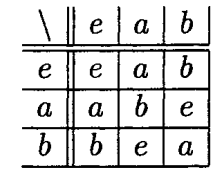
\includegraphics[width=0.3\textwidth]{figures/z3-group.png}
    \caption{Z$_3$ group multiplication table. (Every row and column
    of the multiplication table contains each element of the group exactly once.
    This must be the case because the inverse exists.)}
\end{figure}

A group G is \textbf{finite} if it has a finite number of elements. Otherwise it is \textbf{infinite}.
The number of elements in a finite group G is called the \textbf{order} of G. For eg: Z$_3$, the cyclic group of order 3.

An \textbf{Abelian group} G in one in which the multiplication law is commutative i.e.
g$_1$g$_2$ = g$_2$g$_1$. And the one which doesn't follows commutation is called \textbf{non-Abelian group}.

\subsection{Representation}
A \textbf{Representation} of a group G is a mapping D of the elements of G onto a set of
linear operators with the following properties:

1. D(\textit{e}) = 1, where 1 is the identity operator in the space on which
the linear operators act. \\
2. D(g$_1$)D(g$_2$) = D(g$_1$g$_2$) i.e. the group multiplication law 
is mapped onto the natural multiplication in the linear space on which the linear operators act.

For eg: representation of Z$_3$ is,
\begin{equation}
    D(e) = 1, \hspace{1cm} D(a) = e^{2\pi i/3}, \hspace{1cm} D(b) = e^{4\pi i/3}
\end{equation}
another representation of Z$_3$ can be directly constructed from the multiplication table as,
\begin{equation}
    D(e) = \begin{pmatrix}
        1 & 0 & 0 \\ 
        0 & 1 & 0 \\ 
        0 & 0 & 1 \\ 
   \end{pmatrix}, \hspace{1cm} 
   D(a) = \begin{pmatrix}
        0 & 0 & 1 \\ 
        1 & 0 & 0 \\ 
        0 & 1 & 0 \\ 
   \end{pmatrix}, \hspace{1cm} 
   D(b) = \begin{pmatrix}
        0 & 1 & 0 \\ 
        0 & 1 & 1 \\ 
        1 & 0 & 0 \\ 
\end{pmatrix},
\end{equation}

By taking the group elements themselves to form an orthonormal basis for a vector space, 
$|e \rangle$, $|a\rangle$, and $|b\rangle$ we can also define \textbf{regular representation} as,
\begin{equation}
    D(g_1)|g_2\rangle = |g_1g_2\rangle
    \label{eqn:representation}
\end{equation}

The \textbf{dimension of a representation} is the dimension of the space on which
it acts and the dimension of the regular representation is the order of the group. The representation of Z$_3$ is 1 dimensional.
For any finite group, we can define a vector space in which the basis vectors are labeled by the group elements.
Then equation \ref{eqn:representation} defines the regular representation.

\subsection{Conjugacy Class}
Conjugacy in abstract algebra is analogous to similarity transformation in linear algebra
which relates the linear transformations behaving in similar fashion under change of basis,
Let G be a group and \textit{g}, \textit{h} $\epsilon$ G. We say \textit{g} and \textit{h} are conjugate,
\textit{g} $\sim$ \textit{h} if $\exists$ \textit{x} $\epsilon$ G s.t. 
\begin{equation}
    h = xgx^{-1} 
\end{equation}

This implies conjugacy is an \textbf{equivalence relation}. Its equivalence classes are called \href{https://www.youtube.com/watch?v=yOt3ppQGuto}{\textbf{conjugacy classes}}.

\subsection{Subgroup}
A group H whose elements are all elements of a group G is called a subgroup of G. 
The identity, and the group G are trivial subgroups of G. For eg., the permutation group S3, has a Z3 subgroup formed by the elements \{e, a$_1$, a$_2$\}. 
Subgroup can be used to divide up the elements of the group into subsets called \href{https://en.wikipedia.org/wiki/Coset}{\textbf{cosets}}.
Given an element \textit{g} of G, the \textbf{left cosets} of H in G are the sets obtained by multiplying each element of H by a fixed element \textit{g} of G (where \textit{g} is the \textbf{left factor})
\begin{center}
    \textit{g}H = \{\textit{g}h : h $\epsilon$ H\} $\forall$ \textit{g} $\epsilon$ G.
\end{center}
The \textbf{right cosets} can be defined similarly where g is now a \textbf{right factor}.
\begin{center}
    H\textit{g} = \{h\textit{g} : h $\epsilon$ H\} $\forall$ \textit{g} $\epsilon$ G.
\end{center}

The number of elements in each coset is the order of H. Every element of G
must belong to one and only one coset. Thus for finite groups, the order of
a subgroup H must be a factor of order of G. 
A subgroup H of G is called an \textbf{invariant} or \textbf{normal subgroup} if $\forall$ g$\epsilon$G
\begin{equation}
    gH = Hg
\end{equation}

i.e.$\forall$ \textit{g} $\epsilon$G and \textit{h}$_1 \: \epsilon$ H $\exists$ an \textit{h}$_2 \: \epsilon$ H s.t.
\begin{center}
    \textit{h}$_1$\textit{g} = \textit{gh}$_2$, or \textit{gh}$_2$\textit{g}$^{-1}$ = \textit{h}$_2$.
\end{center} 

The trivial subgroups e and G are invariant for any group. If H is invariant then H\textit{g}$_1$ H\textit{g}$_1^{-1}$ = H, 
so the product of elements in two cosets is in the coset represented by the product of the elements. 
In this case, the coset space G/H, is called the \textbf{factor group} of G by H.

The \textbf{center} of a group G is the set of all elements of G that commute
with all elements of G. The center is always an Abelian, invariant subgroup
of G. However, it may be trivial, consisting only of the identity, or of the
whole group.


The \textbf{characters} $\chi_D$(g) of a group representation D are the traces of the linear
operators of the representation or their matrix elements:
\begin{equation}
    \chi_D(g) \equiv Tr D(g) = \sum_{i}[D(g)]_{ii}
\end{equation}

The advantage of the characters is that because of the cyclic property of the trace Tr(AB) = Tr(BA), they are unchanged by similarity transformations,
thus all equivalent representations have the same characters. The characters are also different for each inequivalent irreducible representation, D$_a$\textemdash 
in fact, they are orthonormal up to an overall factor of N.

\subsection{Eigenstates}
In quantum mechanics, we are often interested in the eigenstates of an invariant hermitian operator, in particular the Hamiltonian, H. 
We can always take these eigenstates to transform according to irreducible representations of the symmetry group. 
To prove this, note that we can divide up the Hilbert space into subspaces with different eigenvalues of H. 
Each subspace furnishes a representation of the symmetry group because D(\textit{g}), the group representation on the full Hilbert space, 
cannot change the H eigenvalue because [D(\textit{g}), H] = 0. But then we can completely reduce the representation in each subspace.
If some irreducible representation appears only once in the Hilbert space, then the states in that representation must be eigenstates
of H (and any other invariant operator). This is true because H$|a, j, x\rangle$ must be in the same irreducible representation, thus
\begin{equation}
    H|a, j, x\rangle = \sum_{y} c_y |a, j, x\rangle
\end{equation}
and if x andy take only one value, then $|a, j, x\rangle$ is an eigenstate.

\textbf{Theorem:} If a hermitian operator H, commutes with all the elements D(\textit{g}), of a representation of the group G, 
then you can choose the eigenstates of H to transform according to irreducible representations of G. 
If an irreducible representation appears only once in the Hilbert space, every state in the irreducible representation 
is an eigenstate of H with the same eigenvalue.

For Abelian groups, this procedure of choosing the H eigenstates to transform under irreducible representations is analogous to simulta-
neously diagonalizing H and D(\textit{g}) because for an Abelian group that commutes with the H, the group elements can simultaneously
diagonalized along with H. This is a consequence of theorem,

\textbf{Theorem:} All of the irreducible representations of a finite Abelian group are 1-dimensional.

For a non-Abelian group, we cannot simultaneously diagonalize all of the D(\textit{g})s, 
but we can completely reduce the representation on each subspace of constant H.
A classical problem which is quite analogous to the problem of diagonalizing the Hamiltonian  in quantum mechanics 
is the problem of finding the normal modes of small oscillations of a mechanical system about a point of stable equilibrium. 
Here, the square of the angular frequency is the eigen value of the M$^{-1}$K matrix and the normal modes are the eigenvectors of M$^{-1}$K.






\subsection{Lie Group}
\href{https://aimath.org/E8/liegroup.html#:~:text=Lie%20groups%20lie%20at%20the,are%20examples%20of%20smooth%20manifolds.}{Lie group}
The definition above is easy to use, but it is not defined for Lie groups that are not matrix groups,  and it is not clear that the \href{https://en.wikipedia.org/wiki/Lie_group}{exponential map}
of a Lie group does not depend on its representation as a matrix group. 
We can solve both problems using a more abstract definition of the exponential map that works for all Lie groups.


\newpage
